\documentclass[aspectratio=169,10pt]{beamer}
\usepackage{amsmath,amssymb}
\usepackage{booktabs}
\usepackage{graphicx}
\usepackage{listings}
\usepackage{xcolor}
\usepackage{hyperref}

% Theme
\usetheme{Madrid}
\usecolortheme{default}

% Title info
\title{Normalization Techniques \& Attention Mechanisms}
\subtitle{CS290W LLM06 Lecture}
\author{LU Yuzhou}
\date{}

% Code listing style
\definecolor{codebg}{RGB}{245,245,245}
\lstset{
    backgroundcolor=\color{codebg},
    basicstyle=\ttfamily\scriptsize,
    frame=single,
    breaklines=true,
    keywordstyle=\color{blue},
    commentstyle=\color{gray},
    stringstyle=\color{red},
    showstringspaces=false,
    upquote=true,
    literate={__}{{\texttt{\_}\texttt{\_}}}2
             {->}{{$\to$}}2
             {=>}{{$\Rightarrow$}}2,
}

\begin{document}

% Title slide
\frame{\titlepage}

% Slide 1: Overview
\begin{frame}{Lecture Overview}
	This lecture covers two foundational building blocks of Transformers:

	\vspace{0.3cm}
	\textbf{Part 1 — Normalization Techniques}
	\begin{itemize}
		\item Why normalization is necessary for deep networks
		\item LayerNorm vs RMSNorm
		\item Activation functions: ReLU, GELU, SiLU
		\item Feed-Forward Networks (FFN)
		\item Pre-Norm vs Post-Norm architectures
	\end{itemize}

	\vspace{0.3cm}
	\textbf{Part 2 — Attention Mechanisms}
	\begin{itemize}
		\item Self-attention: Query, Key, Value
		\item Scaled dot-product attention
		\item Causal masking for autoregressive models
		\item Multi-head attention
	\end{itemize}
\end{frame}

% ==================== PART 1: NORMALIZATION ====================

\begin{frame}{Part 1: Normalization Techniques}
	\begin{center}
		\Large Why do we need normalization?
	\end{center}
\end{frame}

% Slide 2: Why Normalization?
\begin{frame}{Why Normalization Matters}
	Deep networks suffer from \textbf{internal covariate shift}: the distribution of each layer's inputs changes during training.

	\vspace{0.2cm}
	\begin{block}{Problems Without Normalization}
		\begin{itemize}
			\item \textbf{Activation scale variations}: values range from $-192$ to $+216$ in a small network
			\item \textbf{Gradient flow problems}: vanishing or exploding gradients
			\item \textbf{Training instability}: requires very small learning rates
			\item \textbf{Slow convergence}: takes many epochs to reach good performance
		\end{itemize}
	\end{block}

	\vspace{0.1cm}
	\begin{center}
		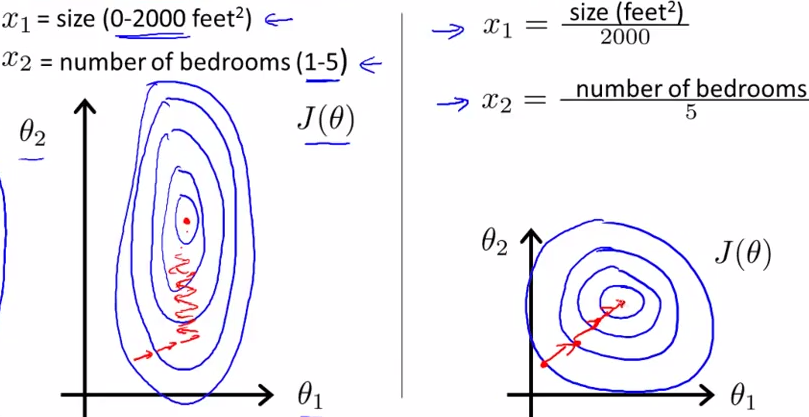
\includegraphics[width=0.45\textwidth]{img/06-01-why-normalization.png}
	\end{center}
\end{frame}

% Slide 3: Layer Normalization
\begin{frame}{Layer Normalization}
	\textbf{LayerNorm} normalizes across the feature dimension for each token position:

	\vspace{0.1cm}
	$$\text{LayerNorm}(x) = \frac{x - \mu}{\sqrt{\sigma^2 + \epsilon}} \cdot \gamma + \beta$$

	\begin{center}
		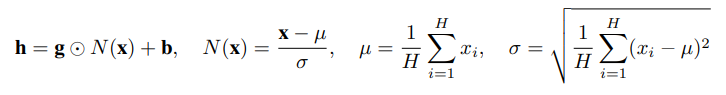
\includegraphics[width=0.65\textwidth]{img/06-02-layernorm-formula.png}
	\end{center}

	\begin{itemize}
		\item $\gamma$ (gain): learnable scaling, initialized to ones
		\item $\beta$ (bias): learnable shifting, initialized to zeros
		\item Output has \textbf{zero mean} and \textbf{unit variance}
	\end{itemize}
\end{frame}

\begin{frame}{Layer Normalization: Diagram}
	\begin{center}
		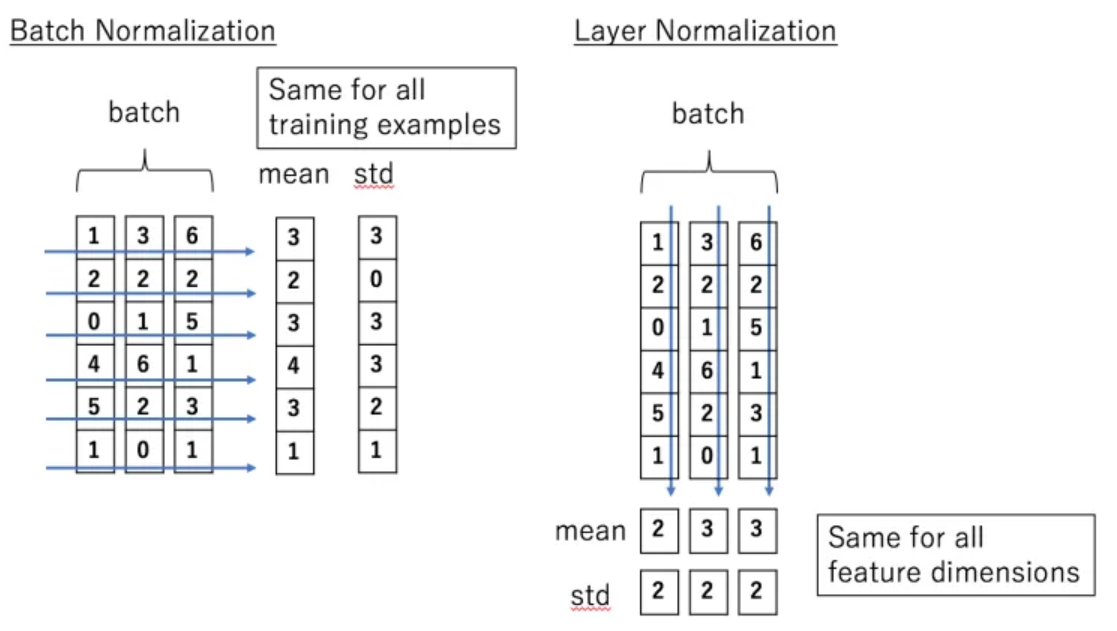
\includegraphics[width=0.6\textwidth]{img/06-03-layernorm-diagram.png}
	\end{center}

	\vspace{0.2cm}
	\begin{block}{Key Property}
		LayerNorm computes $\mu$ and $\sigma$ per-sample, per-position across the feature dimension. \\
		This makes it independent of batch size — ideal for variable-length sequences in LLMs.
	\end{block}
\end{frame}

% Slide 4: RMS Normalization
\begin{frame}{RMS Normalization (RMSNorm)}
	\textbf{RMSNorm} is a simplified alternative to LayerNorm, used in \textbf{LLaMA} and other modern models.

	\vspace{0.1cm}
	$$\text{RMSNorm}(x) = \frac{x}{\text{RMS}(x)} \cdot \gamma, \quad \text{RMS}(x) = \sqrt{\frac{1}{d}\sum_{i=1}^{d} x_i^2 + \epsilon}$$

	\begin{center}
		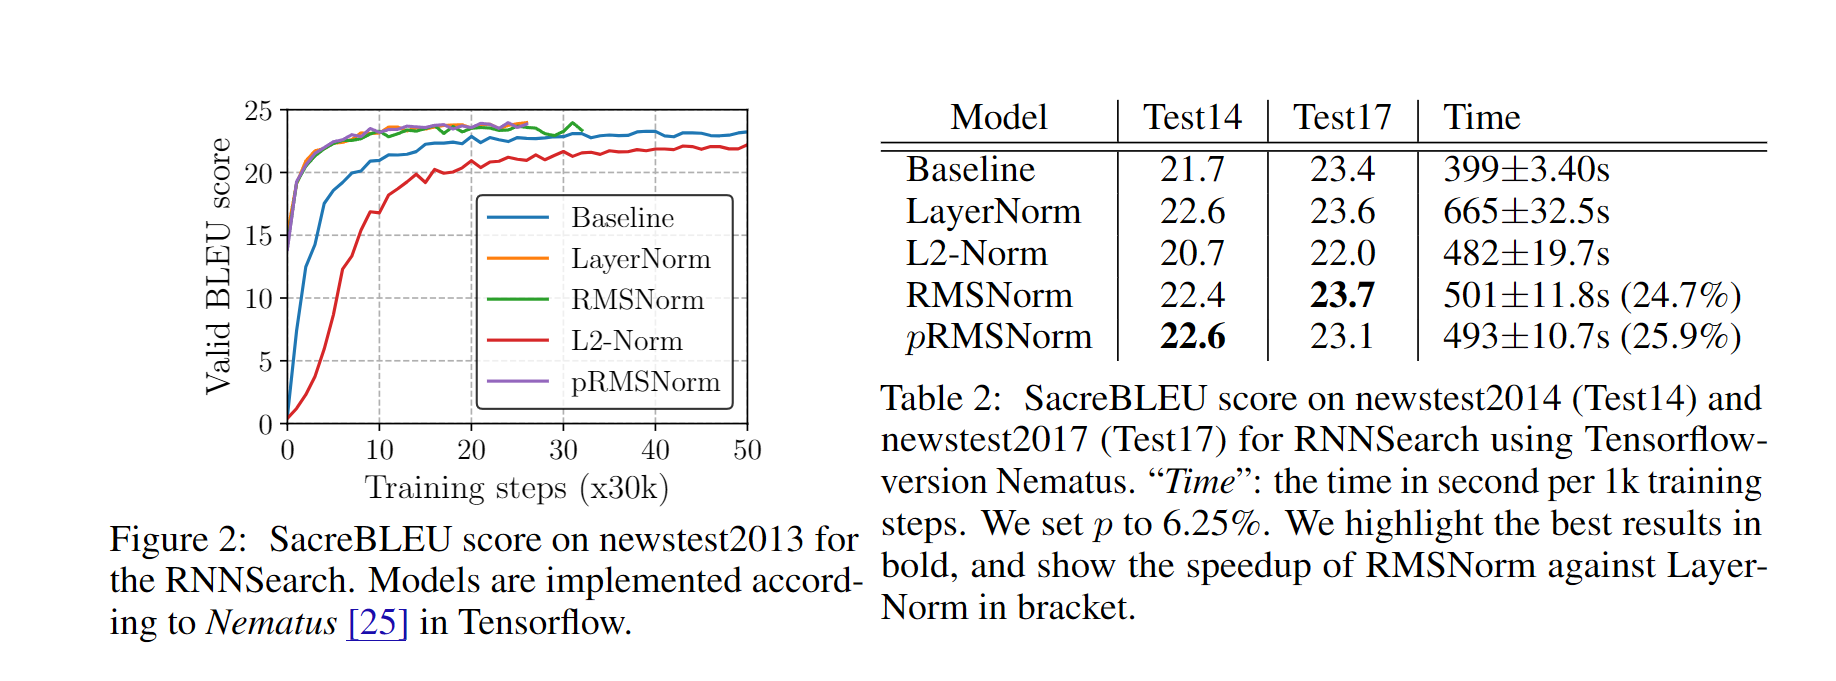
\includegraphics[width=0.6\textwidth]{img/06-04-rmsnorm-formula.png}
	\end{center}

	\begin{itemize}
		\item \textbf{No mean subtraction} — only normalizes by root mean square
		\item \textbf{No bias term} — only a learnable $\gamma$ parameter
		\item $\sim 10$--$30\%$ faster than LayerNorm on GPU
	\end{itemize}
\end{frame}

% Slide 5: RMSNorm Implementation
\begin{frame}[fragile]{RMSNorm: Implementation}
	\begin{lstlisting}[language=Python]
class RMSNorm(nn.Module):
    def __init__(self, dim: int, eps: float = 1e-6):
        super().__init__()
        self.eps = eps
        self.weight = nn.Parameter(torch.ones(dim))

    def _norm(self, x):
        # RMS = sqrt(mean(x^2) + eps)
        rms = x.pow(2).mean(-1, keepdim=True).add(self.eps).sqrt()
        return x / rms

    def forward(self, x):
        output = self._norm(x.float()).type_as(x)
        return output * self.weight
    \end{lstlisting}

	\vspace{0.3cm}
	\begin{itemize}
		\item Cast to \texttt{float32} for numerical stability, then cast back
		\item Only 1 learnable parameter per feature dimension (vs 2 for LayerNorm)
	\end{itemize}
\end{frame}

% Slide 6: LayerNorm vs RMSNorm Comparison
\begin{frame}{LayerNorm vs RMSNorm: Comparison}
	\begin{center}
		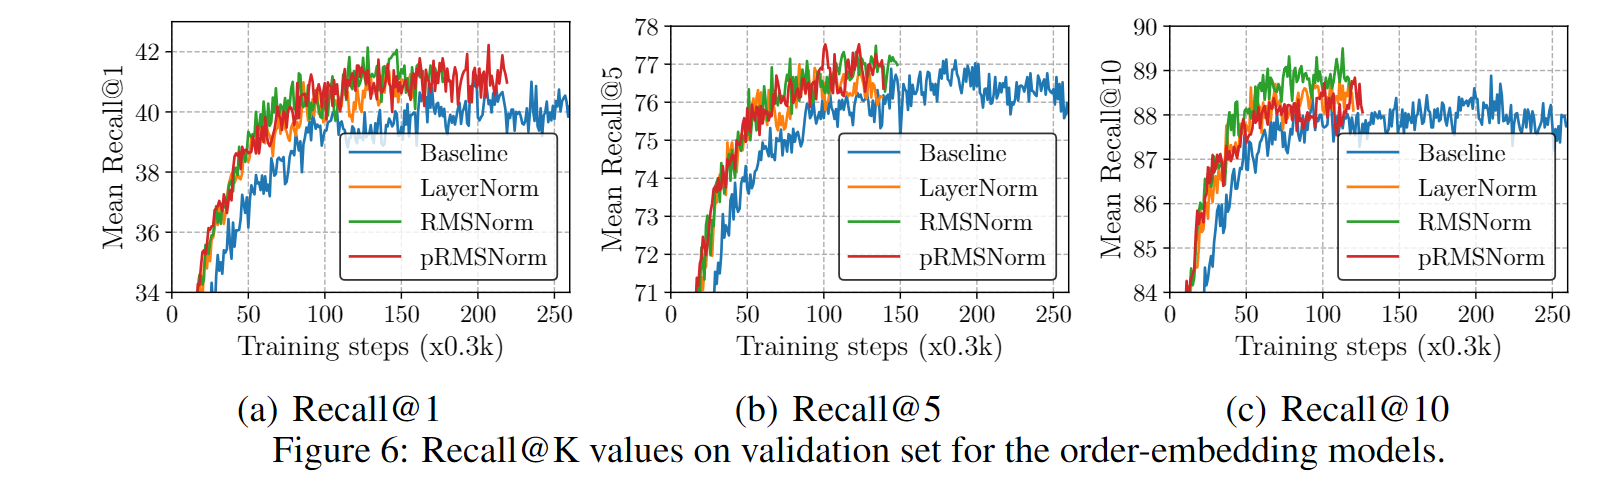
\includegraphics[width=0.6\textwidth]{img/06-05-rmsnorm-comparison.png}
	\end{center}

	\vspace{0.1cm}
	\begin{table}
		\centering
		\small
		\begin{tabular}{lcc}
			\toprule
			\textbf{Property}      & \textbf{LayerNorm} & \textbf{RMSNorm}          \\
			\midrule
			Mean subtraction       & Yes                & No                        \\
			Variance normalization & Yes                & Yes (RMS)                 \\
			Learnable parameters   & $\gamma, \beta$    & $\gamma$ only             \\
			Output mean            & $\approx 0$        & Preserved                 \\
			GPU speed              & Baseline           & $1.1$--$1.3\times$ faster \\
			\midrule
			Used in                & BERT, GPT-2        & LLaMA, Mistral            \\
			\bottomrule
		\end{tabular}
	\end{table}
\end{frame}

% Slide 7: Activation Functions
\begin{frame}{Activation Functions in Modern LLMs}
	Activation functions introduce \textbf{non-linearity}, enabling models to learn complex patterns.

	\begin{center}
		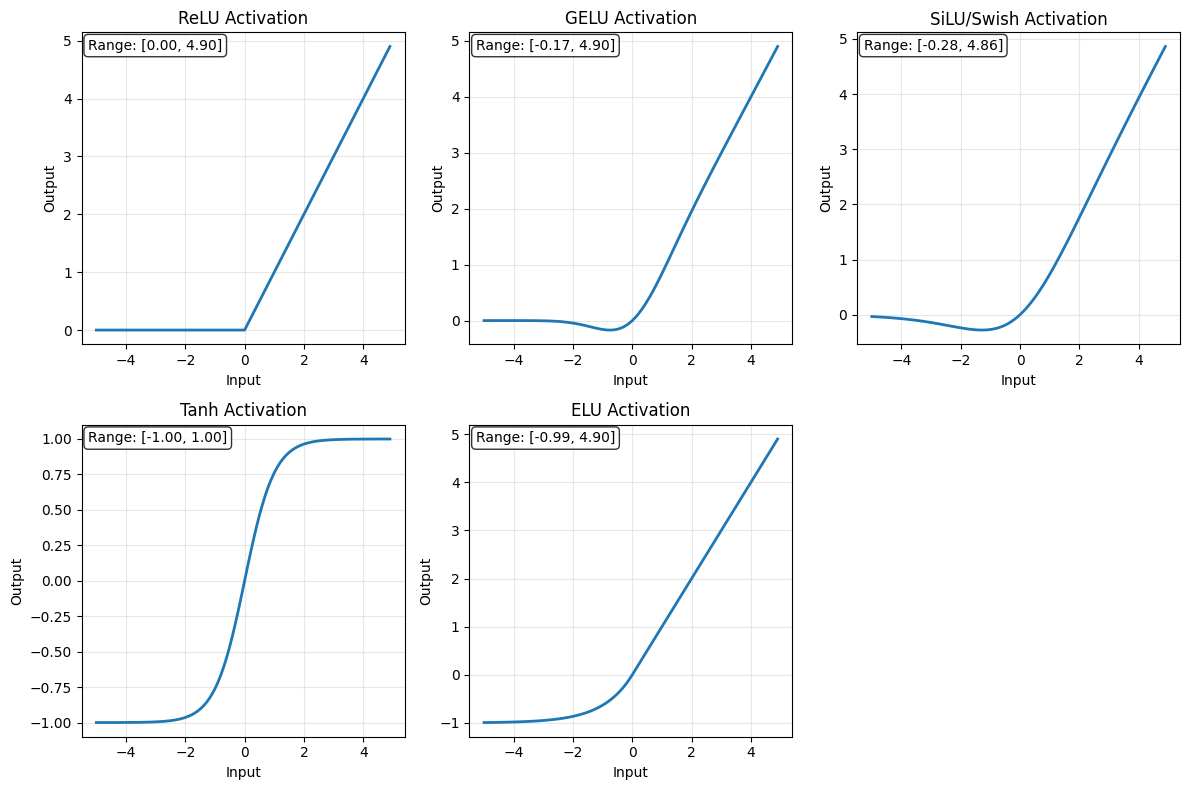
\includegraphics[width=0.55\textwidth]{img/06-06-activation-functions.png}
	\end{center}

	\vspace{0.1cm}
	\begin{table}
		\centering
		\small
		\begin{tabular}{llll}
			\toprule
			\textbf{Function} & \textbf{Formula}    & \textbf{Gradient} & \textbf{Used In} \\
			\midrule
			ReLU              & $\max(0, x)$        & $0$ or $1$        & Classic models   \\
			GELU              & $x \cdot \Phi(x)$   & Smooth            & BERT, GPT-2      \\
			SiLU/Swish        & $x \cdot \sigma(x)$ & Smooth            & LLaMA            \\
			\bottomrule
		\end{tabular}
	\end{table}
\end{frame}

% Slide 8: Feed-Forward Network
\begin{frame}{Feed-Forward Network (FFN) in Transformers}
	Each Transformer block contains an FFN after the attention layer:

	\vspace{0.3cm}
	$$\text{FFN}(x) = W_2 \cdot \text{activation}(W_1 x + b_1) + b_2$$

	\vspace{0.2cm}
	\begin{itemize}
		\item $W_1$: up-projection, $d_{\text{model}} \to d_{\text{ff}}$ (typically $4\times$ expansion)
		\item $W_2$: down-projection, $d_{\text{ff}} \to d_{\text{model}}$
		\item Activation: GELU (BERT, GPT-2) or SiLU (LLaMA)
	\end{itemize}

	\vspace{0.3cm}
	\begin{block}{Design Choices}
		\begin{itemize}
			\item Expansion ratio: typically $4\times$ (e.g., 768 $\to$ 3072 in BERT)
			\item FFN contains \textbf{most parameters} in a Transformer block
			\item Dropout for regularization (typically $p=0.1$)
			\item Residual connections prevent vanishing gradients
		\end{itemize}
	\end{block}
\end{frame}

% Slide 9: Pre-Norm vs Post-Norm
\begin{frame}{Pre-Norm vs Post-Norm Architectures}
	The \textbf{placement} of normalization significantly impacts training dynamics.

	\begin{center}
		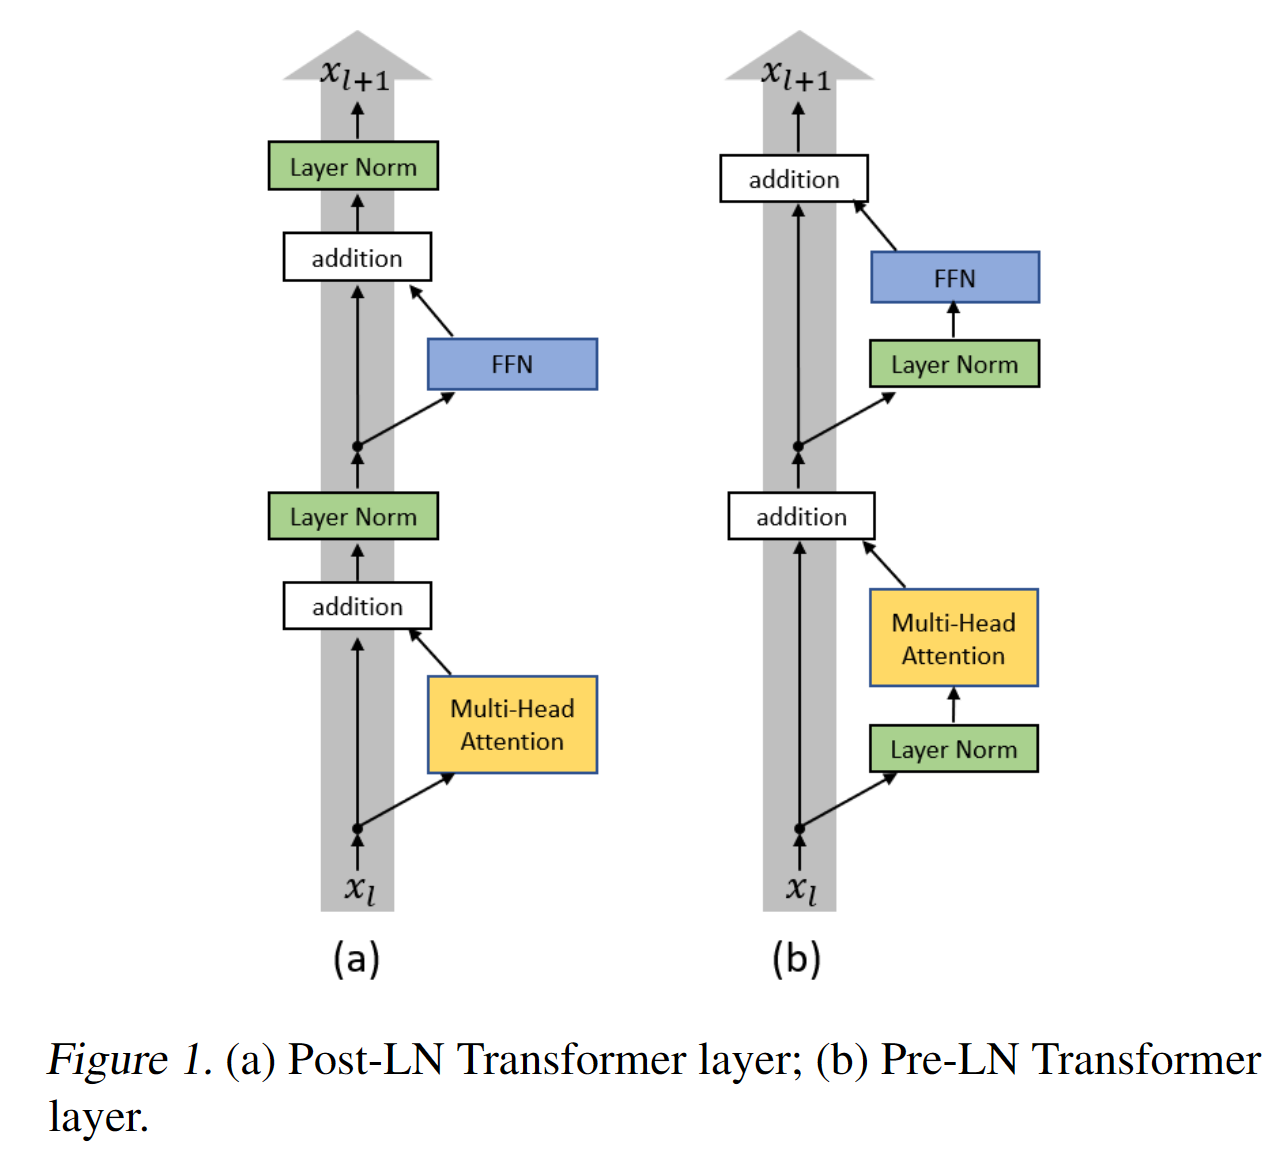
\includegraphics[width=0.55\textwidth]{img/06-07-prenorm-postnorm.png}
	\end{center}

	\vspace{0.1cm}
	\begin{table}
		\centering
		\small
		\begin{tabular}{lcc}
			\toprule
			                  & \textbf{Post-Norm}      & \textbf{Pre-Norm}       \\
			\midrule
			Gradient flow     & Can vanish in deep nets & More stable             \\
			Training          & Requires careful warmup & Easier to train         \\
			Final performance & Often slightly better   & Good                    \\
			Scalability       & Hard for $>24$ layers   & Preferred for deep LLMs \\
			\bottomrule
		\end{tabular}
	\end{table}
\end{frame}

\begin{frame}{Pre-Norm vs Post-Norm: Detailed Comparison}
	\begin{center}
		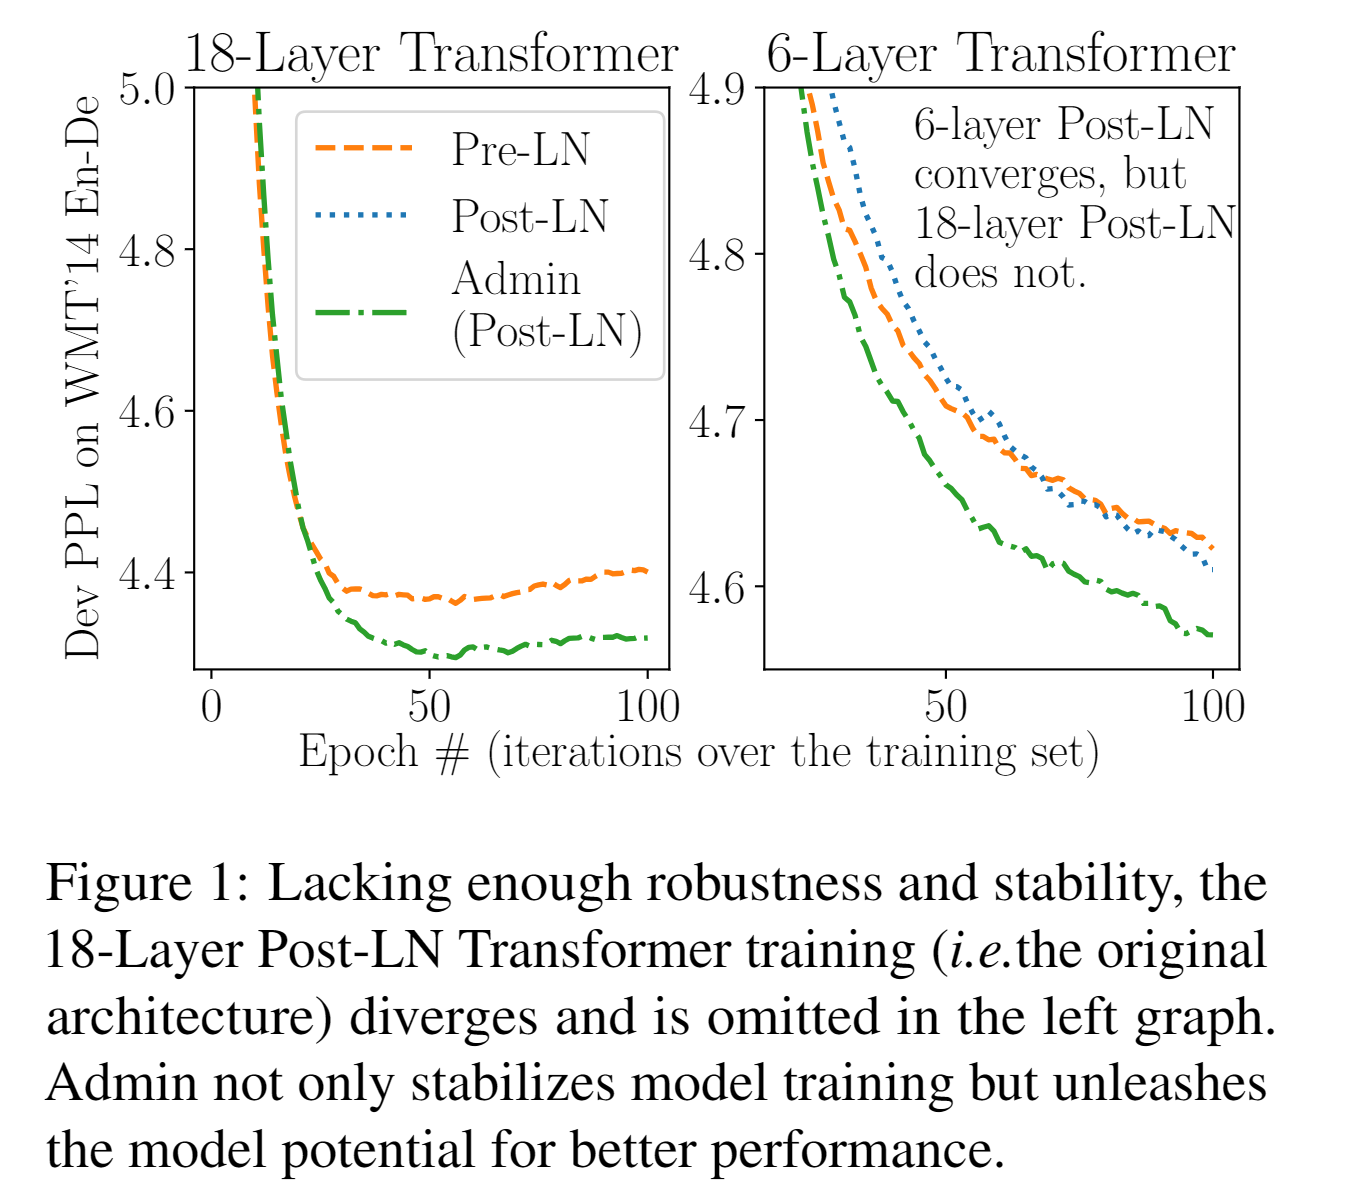
\includegraphics[width=0.55\textwidth]{img/06-08-prenorm-postnorm-compare.png}
	\end{center}

	\vspace{0.2cm}
	\begin{block}{Key Insight}
		Pre-Norm keeps a \textbf{clean residual path} from input to output, improving gradient flow in deep networks. \\
		Most modern LLMs (GPT-2/3, LLaMA, Mistral) use Pre-Norm with RMSNorm.
	\end{block}
\end{frame}

% Slide 10: Pre-Norm vs Post-Norm Code
\begin{frame}[fragile]{Pre-Norm vs Post-Norm: Code}
	\textbf{Post-Norm:}
	\begin{lstlisting}[language=Python]
def forward(self, x):
    # Attention: apply, add residual, normalize
    x = self.ln1(x + self.attention(x))
    # FFN: apply, add residual, normalize
    x = self.ln2(x + self.ffn(x))
    return x
    \end{lstlisting}

	\vspace{0.3cm}
	\textbf{Pre-Norm:}
	\begin{lstlisting}[language=Python]
def forward(self, x):
    # Attention: normalize, apply, add residual
    x = x + self.attention(self.ln1(x))
    # FFN: normalize, apply, add residual
    x = x + self.ffn(self.ln2(x))
    return x
    \end{lstlisting}

	\vspace{0.3cm}
	\begin{block}{Key Insight}
		Pre-Norm keeps a \textbf{clean residual path} from input to output, improving gradient flow in deep networks.
	\end{block}
\end{frame}

% ==================== PART 2: ATTENTION ====================

\begin{frame}{Part 2: Attention Mechanisms}
	\begin{center}
		\Large The Heart of Transformers
	\end{center}
\end{frame}

% Slide 11: What is Attention?
\begin{frame}{Self-Attention: The Big Idea}
	Self-attention allows each position in a sequence to \textbf{attend to all other positions}.

	\begin{center}
		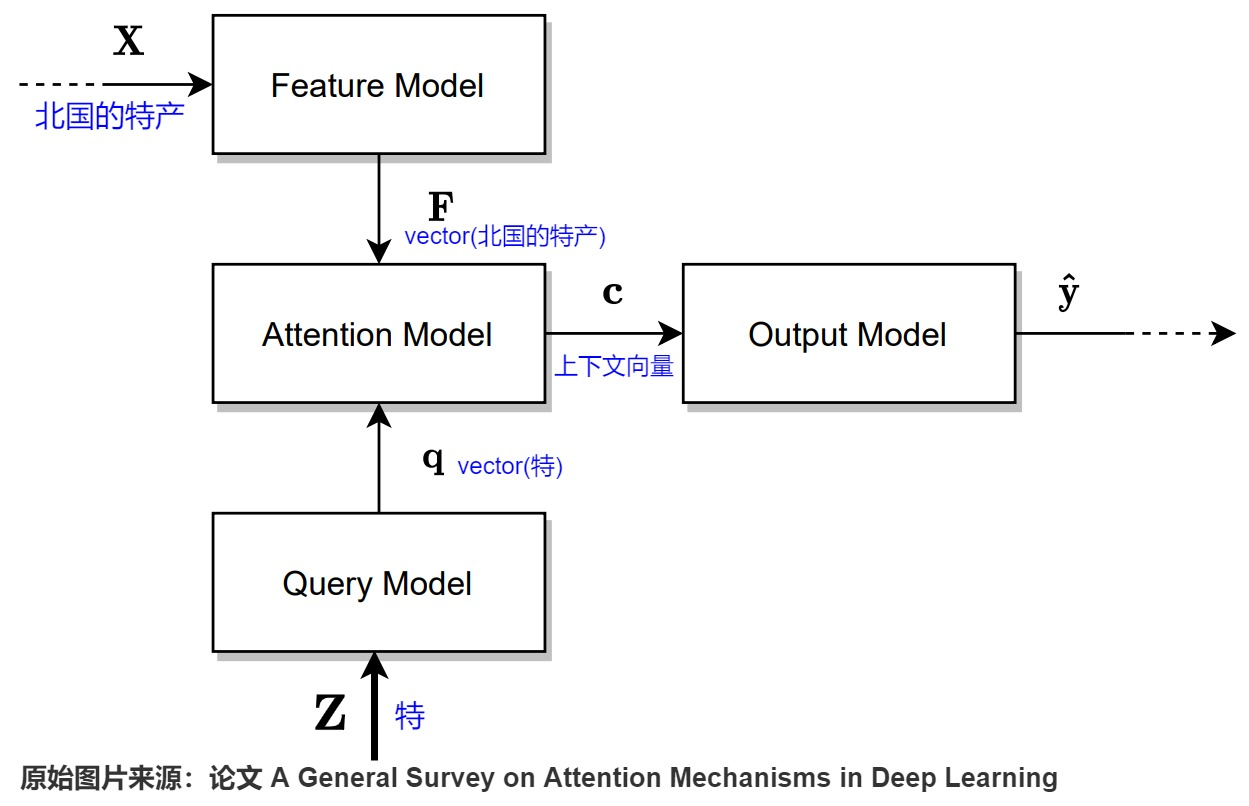
\includegraphics[width=0.38\textwidth]{img/06-09-attention-intro1.jpg}
		\hfill
		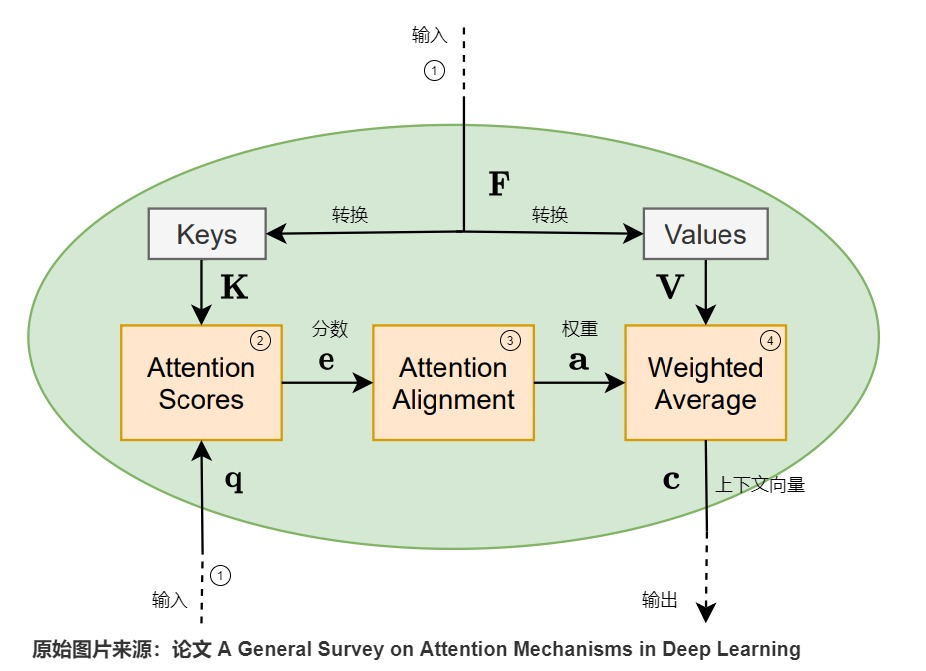
\includegraphics[width=0.38\textwidth]{img/06-10-attention-intro2.jpg}
	\end{center}

	\vspace{0.1cm}
	\textbf{Three roles per token:}
	\begin{itemize}
		\item \textbf{Query (Q)}: ``What am I looking for?'' — what information does this position need?
		\item \textbf{Key (K)}: ``What do I have to offer?'' — what information does this position contain?
		\item \textbf{Value (V)}: ``What do I actually give?'' — the actual content to be shared
	\end{itemize}

	$$Q = XW_Q, \quad K = XW_K, \quad V = XW_V$$
\end{frame}

% Slide 12: Attention Score Computation
\begin{frame}{Scaled Dot-Product Attention}
	\begin{center}
		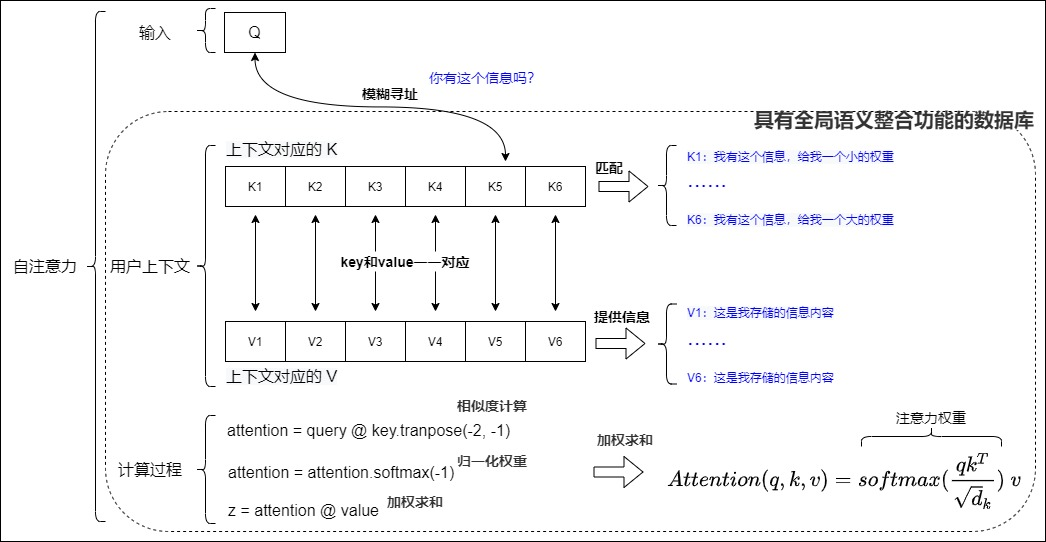
\includegraphics[width=0.45\textwidth]{img/06-11-attention-mechanism.jpg}
	\end{center}

	$$\text{Attention}(Q, K, V) = \text{softmax}\!\left(\frac{QK^T}{\sqrt{d_k}}\right) V$$

	\textbf{Step-by-step:}
	\begin{enumerate}
		\item \textbf{Compute scores}: $S = QK^T$ — dot product measures similarity
		\item \textbf{Scale}: $S / \sqrt{d_k}$ — prevent extremely large values
		\item \textbf{Mask} (optional): set forbidden positions to $-\infty$
		\item \textbf{Softmax}: convert scores to probabilities (rows sum to 1)
		\item \textbf{Weighted sum}: $O = \text{softmax}(S) \cdot V$
	\end{enumerate}
\end{frame}

% Slide 13: Attention Intuition
\begin{frame}{Attention Score Intuition}
	Consider the sentence: ``\textit{The cat sat on the mat because \underline{it} was tired}''

	\vspace{0.3cm}
	\begin{itemize}
		\item When processing ``\textit{it}'', the model needs to know \textit{what} ``it'' refers to
		\item The Query of ``\textit{it}'' asks: ``Who is the subject?''
		\item The Key of ``\textit{cat}'' says: ``I am a noun, potentially a subject''
		\item High $Q \cdot K$ score → ``\textit{it}'' attends strongly to ``\textit{cat}''
		\item The Value of ``\textit{cat}'' flows into ``\textit{it}'' representation
	\end{itemize}

	\vspace{0.3cm}
	\begin{block}{Key Insight}
		Attention scores form a \textbf{probability distribution} over all positions. \\
		Higher scores = more information flow between those positions.
	\end{block}
\end{frame}

% Slide 14: Causal Masking
\begin{frame}{Causal Masking for Autoregressive Models}
	\begin{center}
		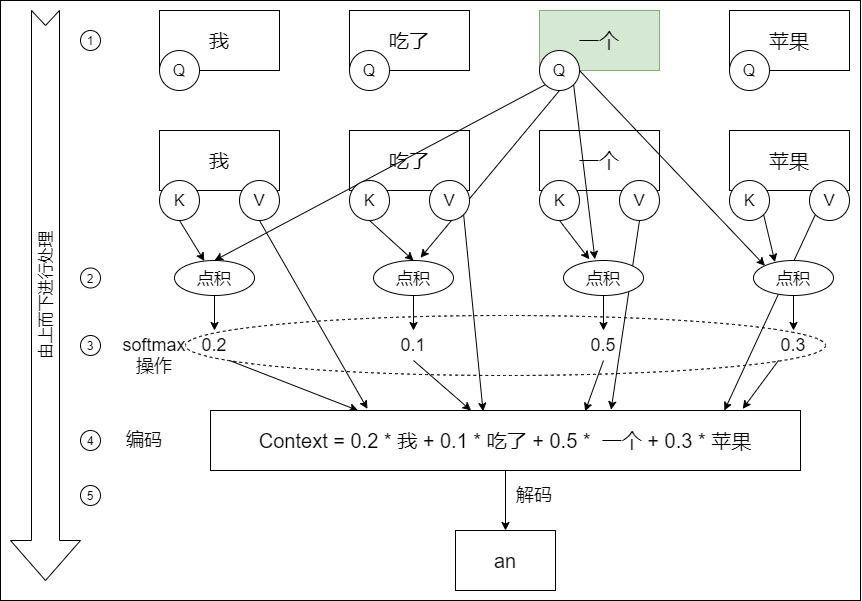
\includegraphics[width=0.45\textwidth]{img/06-12-attention-weights.jpg}
	\end{center}

	\textbf{Problem:} In GPT-style models, position $i$ must \textbf{not see future tokens} $j > i$.

	\textbf{Solution}: Apply a causal mask before softmax:
	$$\text{mask}_{ij} = \begin{cases} 0 & \text{if } j \leq i \\ -\infty & \text{if } j > i \end{cases}$$

	\begin{block}{Effect}
		After softmax, masked positions get $\approx 0$ weight. \\
		Position 0 sees only itself; position $n$ sees all positions $\leq n$.
	\end{block}
\end{frame}

% Slide 15: Padding Mask
\begin{frame}{Padding Mask}
	For variable-length sequences, shorter inputs are padded with special tokens.

	\vspace{0.3cm}
	\begin{itemize}
		\item Padding tokens are \textbf{not real content} — should not receive attention
		\item Set padding positions to $-\infty$ in the attention score matrix
		\item After softmax, padding positions get $\approx 0$ weight
	\end{itemize}

	\vspace{0.3cm}
	\begin{lstlisting}[language=Python]
# Example: position 2 is padded in batch element 1
padding_mask = torch.zeros(batch_size, seq_len).bool()
padding_mask[1, 2] = True  # Mark as padded

# Apply mask: set padded positions to -inf
scores[padding_mask.unsqueeze(1).expand(-1, seq_len, -1)] = float('-inf')
    \end{lstlisting}

	\vspace{0.3cm}
	\begin{block}{Multiple Masks}
		Causal and padding masks can be \textbf{combined} for autoregressive models with variable-length inputs.
	\end{block}
\end{frame}

% Slide 16: Multi-Head Attention
\begin{frame}{Multi-Head Attention}
	\begin{center}
		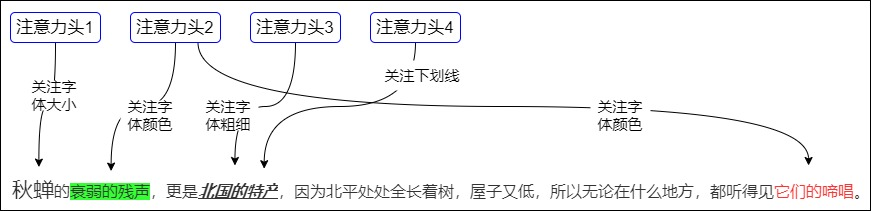
\includegraphics[width=0.38\textwidth]{img/06-14-multihead-overview.jpg}
		\hfill
		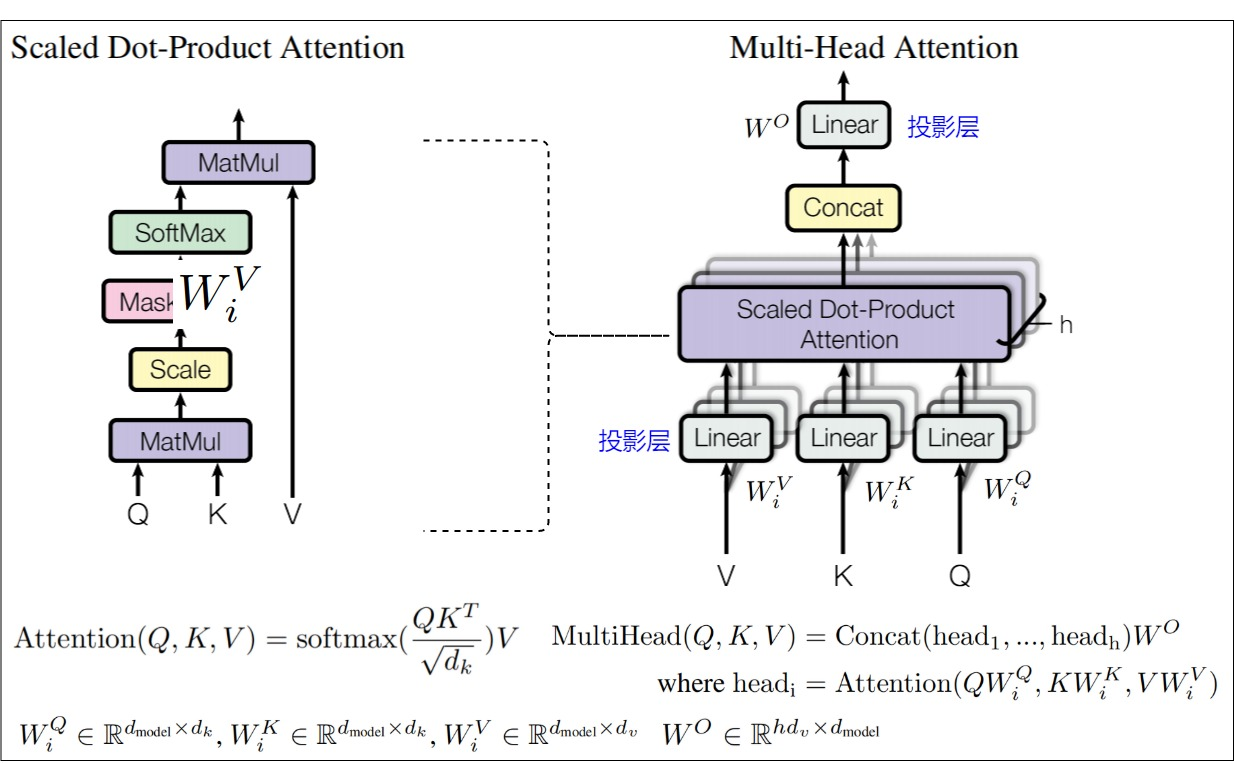
\includegraphics[width=0.38\textwidth]{img/06-15-multihead-detail.jpg}
	\end{center}

	$$\text{MultiHead}(Q, K, V) = \text{Concat}(\text{head}_1, \ldots, \text{head}_h) W_O$$
	$$\text{where head}_i = \text{Attention}(QW_i^Q, KW_i^K, VW_i^V)$$

	\begin{itemize}
		\item $h$ heads (e.g., 8 or 12), $\text{head\_dim} = d_{\text{model}} / h$
		\item Different heads learn \textbf{different relationship types} (syntax, semantics, position)
		\item Parallel computation → efficient on GPU
	\end{itemize}
\end{frame}

% Slide 17: Multi-Head Attention Implementation
\begin{frame}[fragile]{Multi-Head Attention: Reshaping}
	Reshape tensors to process all heads simultaneously:

	\vspace{0.3cm}
	\begin{lstlisting}[language=Python]
# Q, K, V shape: [batch, seq_len, hidden_dim]
# e.g., [2, 4, 8] with num_heads=2, head_dim=4

# Step 1: Reshape [batch, seq, hidden] -> [batch, seq, heads, head_dim]
q_heads = q.view(batch_size, seq_len, num_heads, head_dim)

# Step 2: Transpose [batch, seq, heads, dim] -> [batch, heads, seq, dim]
q_heads = q_heads.transpose(1, 2)

# Step 3: Compute attention for ALL heads simultaneously
scores = torch.matmul(q_heads, k_heads.transpose(-2, -1))
scores = scores / math.sqrt(head_dim)
weights = F.softmax(scores + causal_mask, dim=-1)
output = torch.matmul(weights, v_heads)

# Step 4: Concatenate heads back
output = output.transpose(1, 2).contiguous().view(batch, seq, hidden)
    \end{lstlisting}
\end{frame}

% Slide 18: Attention Visualization
\begin{frame}{Visualizing Attention Patterns}
	\begin{center}
		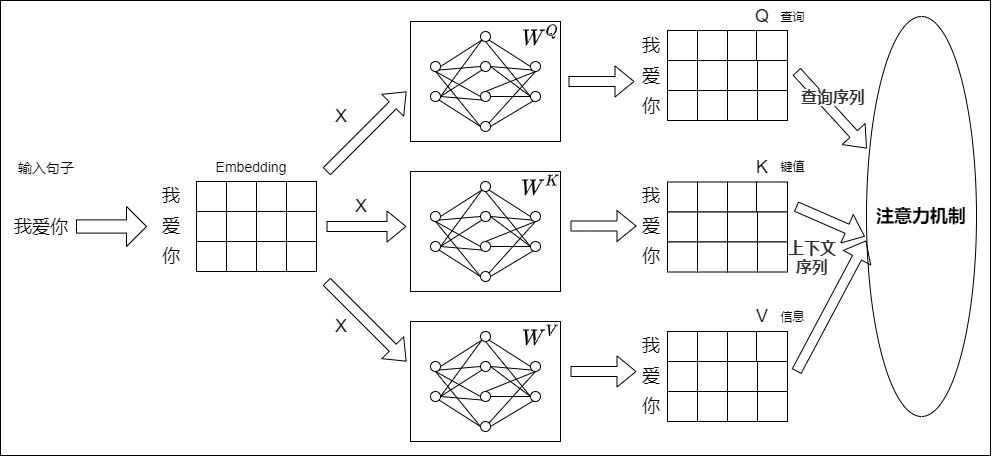
\includegraphics[width=0.5\textwidth]{img/06-13-attention-matrices.jpg}
	\end{center}

	\vspace{0.1cm}
	\begin{itemize}
		\item Each head produces a different attention pattern
		\item Some heads attend to \textbf{local context} (nearby tokens)
		\item Some heads attend to \textbf{long-range dependencies}
		\item Some heads focus on specific \textbf{syntactic patterns}
	\end{itemize}

	\textbf{Interpretability:} Attention weights show which tokens the model ``focuses on'' for each position.
\end{frame}

% Slide 19: Output Projection
\begin{frame}{Output Projection and Complete Pipeline}
	After multi-head attention, apply a final linear projection:

	$$\text{output} = W_O \cdot \text{MultiHead}(Q, K, V)$$

	\textbf{Complete attention pipeline:}
	\begin{enumerate}
		\item Input $X \in \mathbb{R}^{B \times N \times d}$
		\item Project to $Q, K, V$ via $W_Q, W_K, W_V$
		\item Reshape for multi-head: $[B, N, d] \to [B, h, N, d/h]$
		\item Compute scaled dot-product attention with causal mask
		\item Concatenate heads: $[B, h, N, d/h] \to [B, N, d]$
		\item Final projection: $W_O$
	\end{enumerate}

	\begin{block}{Complexity}
		$O(N^2 d)$ — quadratic in sequence length $N$, linear in hidden dim $d$.
	\end{block}
\end{frame}

% Slide 20: Summary
\begin{frame}{Summary: Key Takeaways}
	\begin{center}
		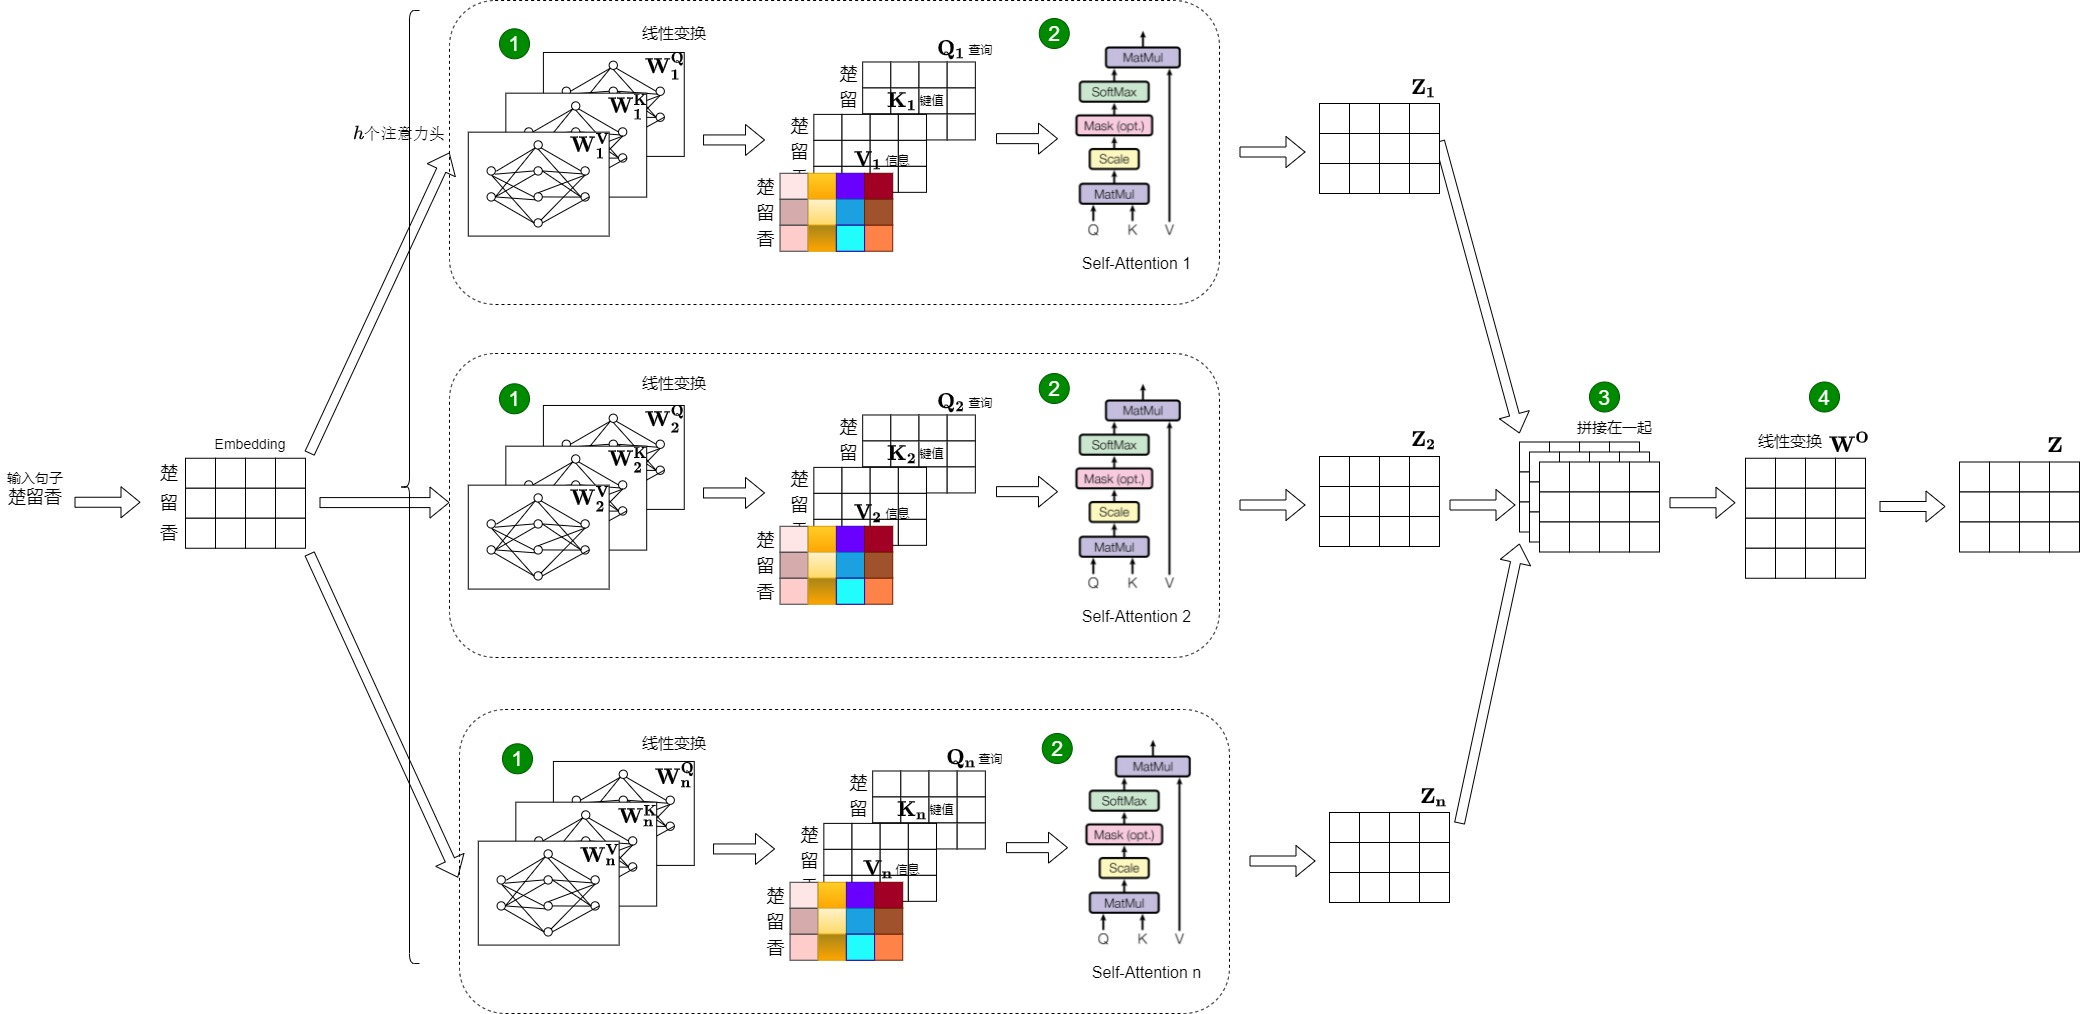
\includegraphics[width=0.55\textwidth]{img/06-16-summary.jpg}
	\end{center}

	\vspace{0.1cm}
	\textbf{Normalization:} LayerNorm (BERT, GPT-2) vs RMSNorm (LLaMA, Mistral); Pre-Norm preferred for deep LLMs.

	\textbf{Attention:} Q/K/V projections $\to$ scaled dot-product $\to$ causal masking $\to$ multi-head $\to$ output projection.

	\vspace{0.1cm}
	\begin{block}{Together}
		Normalization + Attention form the \textbf{core building blocks} of every Transformer layer.
	\end{block}
\end{frame}

% Slide 21: Lab Notebooks
\begin{frame}{Lab Notebooks}
	\begin{itemize}
		\item \texttt{LLM05a-Normalization-Techniques.ipynb}
		      \begin{itemize}
			      \item Implement custom RMSNorm
			      \item Compare LayerNorm vs RMSNorm statistics
			      \item Analyze activation functions (ReLU, GELU, SiLU)
			      \item Build Transformer FFN and complete blocks
		      \end{itemize}

		      \vspace{0.2cm}
		\item \texttt{LLM05b-Advanced-Normalization-Applications.ipynb}
		      \begin{itemize}
			      \item Implement LayerNorm from scratch
			      \item Pre-Norm vs Post-Norm architecture comparison
			      \item Gradient flow analysis
		      \end{itemize}

		      \vspace{0.2cm}
		\item \texttt{LLM06-Attention-Mechanisms.ipynb}
		      \begin{itemize}
			      \item Implement Q, K, V projections
			      \item Compute attention scores with scaling and masking
			      \item Build multi-head attention from scratch
			      \item Visualize attention patterns
		      \end{itemize}
	\end{itemize}
\end{frame}

\end{document}
